%%%%%%%%%%%%%%%%%%%%%%%%%%%%%%%%%%%%%%%%%%%%%%%%%%%%%%%%
%%%%%%%%%%%%%%%%%%%%%%%%%%%%%%%%%%%%%%%%%%%%%%%%%%%%%%%%
\section{Statistics}
\label{additional:stats}

%%%%%%%%%%%%%%%%%%%%%%%%%%%%%%%%%%%%%%%%%%%%%%%%%%%%%%%%
\subsection{Expectation Value and Variance}
\label{additional:stats:expval_and_var}

The expectation value \cref{eq:stats:exp_relations} and variance \cref{eq:stats:var_relations} are introductory, yet essential, statistical measures.
Their definitions and interesting properties are reproduced here for reference.
Note that $s$ is the unbiased sample variance,
and the sample mean $\bar{x}$ has $\mu_{\bar{x}} = \mu$, $\sigma_{\bar{x}} = \sigma / \sqrt{n}$,
where $\mu$ and $\sigma$ are from the parent population.

\begin{subequations}\label{eq:stats:exp_relations}
\begin{align}
\expvalE{X} = \expval{X} &= \sum_{j=1}^{m} x_{j} \, p_{j} = \int_{-\infty}^{\infty} x f\left(x\right) \, \dif x \label{eq:stats:exp_relations:def} \\
\bar{x} = \mu &= \frac{1}{n} \sum_{j=1}^{m} x_{j}\,,\,\text{for uniform}~p_{j} \label{eq:stats:exp_relations:mean} \\
\expval{X+Y} &= \expval{X} + \expval{X} \label{eq:stats:exp_relations:add} \\
\expval{a X} &= a \expval{X} \label{eq:stats:exp_relations:mult} \\
\expval{a} &= a \,\, \Rightarrow \, \expval{\expval{X}} = \expval{X} \label{eq:stats:exp_relations:self} \\
\expval{X Y}^{2} &\leq \expval{X^{2}} \expval{Y^{2}} \label{eq:stats:exp_relations:cbs_ineq}
\end{align}
\end{subequations}

\begin{subequations}\label{eq:stats:var_relations}
\begin{align}
\sigma_{X}^{2} = \variance{X} &= \expval{\left(x-\bar{x}\right)^{2}} = \expval{X^{2}} - \expval{X}^{2} \label{eq:stats:var_relations:def} \\
s^{2} &= \frac{1}{n-1} \sum_{j=1}^{m} \left( x_{j} - \bar{x}\right)^{2} \label{eq:stats:var_relations:sample} \\
\variance{X+a} &= \variance{X} \label{eq:stats:var_relations:add} \\
\variance{a X} &= a^{2} \, \variance{X} \label{eq:stats:var_relations:mult} \\
\variance{a X \pm b Y} &= a^{2} \, \variance{X} + b^{2} \, \variance{Y} \pm 2 \, ab \, \cov{X}{Y} \label{eq:stats:var_relations:linear} \\
\variance{X \mid Y} &= \expval{\left(X - \expval{X \mid Y}\right)^{2} \mid Y} \label{eq:stats:var_relations:conditional1} \\
\variance{X} &= \expval{\variance{X \mid Y}} + \variance{\expval{X \mid Y}} \label{eq:stats:var_relations:conditional2}
\end{align}
\end{subequations}

%%%%%%%%%%%%%%%%%%%%%%%%%%%%%%%%%%%%%%%%%%%%%%%%%%%%%%%%
\subsection{Covariance and Correlation}
\label{additional:stats:corr_covar}

The covariance between two variables $u$ and $v$,

\begin{equation}\label{eq:stats:covar}
\begin{split}
\sigma_{u,v}^{2} = \cov{u}{v} &= \frac{1}{m}\sum_{j=1}^{m}\left(u_{j}-\bar{u}\right)\left(v_{j}-\bar{v}\right) \\
&= \expval{\left(u-\bar{u}\right)\left(v-\bar{v}\right)} \\
&= \expval{u v} - \expval{u}\expval{v}\,,
\end{split}
\end{equation}

\noindent is a measure of their joint variability,
\ie a measure of any linear relationship which may exist between them.
It is helpful to remember the following covariance relations:

\begin{subequations}\label{eq:stats:covar_relations}
\begin{align}
\cov{X}{X} &= \variance{X}, \label{eq:stats:covar_relations:var} \\
\cov{X + a}{Y + b} &= \cov{X}{Y}, \label{eq:stats:covar_relations:add} \\
\cov{a\,X}{b\,Y} &= ab\,\cov{X}{Y}. \label{eq:stats:covar_relations:mult}
\end{align}
\end{subequations}
The correlation coefficient,

\begin{equation}\label{eq:stats:corr}
\rho_{u,v} = \frac{\sigma_{u,v}^{2}}{\sigma_{u}\sigma_{v}} = \frac{\cov{u}{v}}{\sigma_{u}\sigma_{v}}\,,
\end{equation}

\noindent is a convenient dimensionless version, normalized to $-1 \leq \rho \leq 1$.
Example distributions can be found in \cref{fig:stats:corr_ex}.

\begin{figure}
\centering
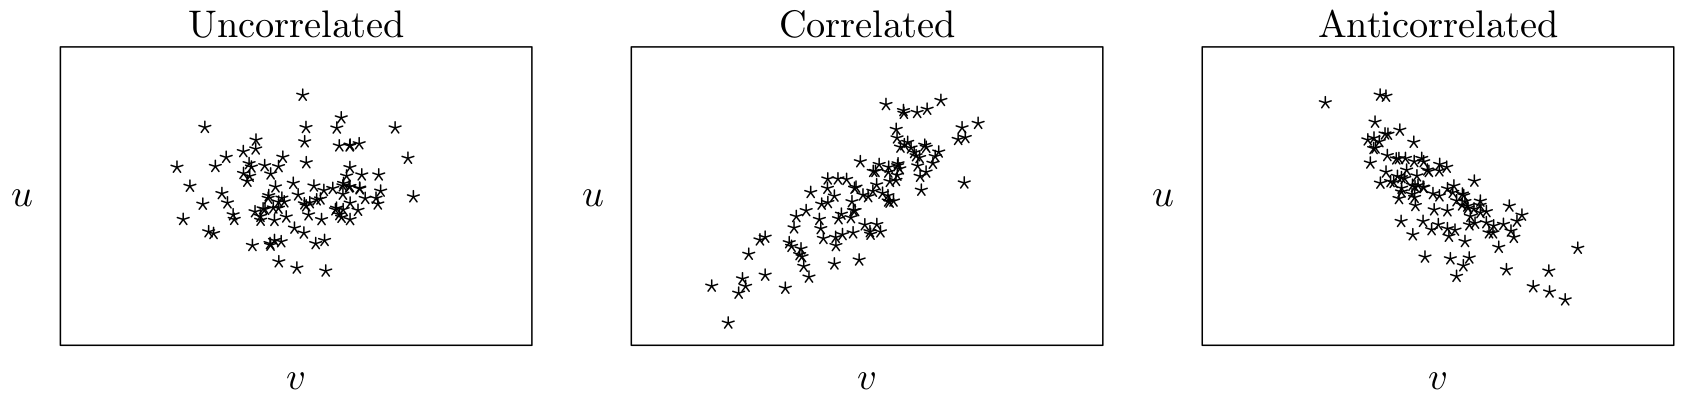
\includegraphics[width=0.95\textwidth]{figures/stats/corr_ex}
\caption{
Example distributions for
uncorrelated ($\rho \approx 0$),
correlated ($\rho \approx 1$),
and anticorrelated ($\rho \approx -1$)
variables $u$ and $v$ \cite{DougNotes}.
}
\label{fig:stats:corr_ex}
\end{figure}

The covariance matrix,

\begin{align}
  \mathbf{M} = \begin{pmatrix}
    \sigma_1^2   & \cov{1}{2} & \cov{1}{3} & \ldots \\
    \cov{1}{2}   & \sigma_2^2 & \cov{2}{3} & \ldots \\
    \cov{1}{3}   & \cov{2}{3} & \sigma_3^2 & \ldots \\
    \vdots       & \vdots     & \vdots     & \ddots
  \end{pmatrix}\,,
\end{align}

\noindent with elements $M_{ij} = \expval{\left(u_{i} - \bar{u}_{i}\right)\left(u_{j}-\bar{u}_{j}\right)}$
is the higher dimensional extension of the covariance.
We can visualize the covariance between variables with
Gaussian error ellipses given by the probability distribution

\begin{equation}\label{eq:stats:P_error_ellipse_k}
P\left(x_{1},x_{2},\ldots,x_{k}\right) = \frac{1}{(2\pi)^{k/2}}\frac{1}{\abs{\mathbf{M}}^{1/2}}\exp\left[-\frac{1}{2}\left(\mathbf{x}-\bm{\mu}\right)^{\transpose}\mathbf{M}\left(\mathbf{x}-\bm{\mu}\right)\right]\,,
\end{equation}

\noindent where the ellipse semi-axes are directed along the eigenvectors of $\mathbf{M}$.
In two dimensions it is easier to see the equation of the error ellipse itself:

\begin{equation}\label{eq:stats:P_error_ellipse_2}
\begin{split}
P\left(u,v\right) &= \frac{1}{2\pi\sigma_{u}\sigma_{v}}\frac{1}{\sqrt{1-\rho^{2}}}\exp\bigg\{-\frac{1}{2}\bigg[ \\
&\frac{1}{(1-\rho)^{2}}\left(\frac{\left(u-\bar{u}\right)^{2}}{\sigma_{u}^{2}}+\frac{\left(v-\bar{v}\right)^{2}}{\sigma_{v}^{2}}-\frac{2\rho \left(u-\bar{u}\right)\left(v-\bar{v}\right)}{\sigma_{u}\sigma_{v}}\right)\bigg]\bigg\}\,.
\end{split}
\end{equation}

%%%%%%%%%%%%%%%%%%%%%%%%%%%%%%%%%%%%%%%%%%%%%%%%%%%%%%%%
\subsection{Bias of a Predictor}
\label{additional:stats:bias}
% TODO

\begin{equation}\label{eq:stats:bias}
\bias{\hat{f}\left(x\right)} = \expval{\hat{f}\left(x\right)} - f\left(x\right)
\end{equation}

%%%%%%%%%%%%%%%%%%%%%%%%%%%%%%%%%%%%%%%%%%%%%%%%%%%%%%%%
\subsection{Principle Component Analysis (PCA)}
\label{additional:stats:PCA}
% TODO

%%%%%%%%%%%%%%%%%%%%%%%%%%%%%%%%%%%%%%%%%%%%%%%%%%%%%%%%
\subsection{Analysis of Variance (ANOVA)}
\label{additional:stats:ANOVA}
% TODO

%%%%%%%%%%%%%%%%%%%%%%%%%%%%%%%%%%%%%%%%%%%%%%%%%%%%%%%%
\subsection{Time Series Analysis}
\label{additional:stats:time_series_ana}
% TODO

%%%%%%%%%%%%%%%%%%%%%%%%%%%%%%%%%%%%%%%%%%%%%%%%%%%%%%%%
\subsection{Kolmogorov-Smirnov Test}
\label{additional:misc:KS_test}
% TODO

%%%%%%%%%%%%%%%%%%%%%%%%%%%%%%%%%%%%%%%%%%%%%%%%%%%%%%%%
\subsection{Kalman Filters}
\label{additional:misc:kalman_filters}
% TODO

%%%%%%%%%%%%%%%%%%%%%%%%%%%%%%%%%%%%%%%%%%%%%%%%%%%%%%%%
\subsection{Markov Chains}
\label{additional:misc:markov_chains}
% TODO

%%%%%%%%%%%%%%%%%%%%%%%%%%%%%%%%%%%%%%%%%%%%%%%%%%%%%%%%
\subsection{Sampling from Probability Distributions}
\label{additional:misc:sampling_prob_dist}
Most programming languages have built-in functions to generate
pseudo-random numbers from common probability distributions,
such as the Poisson \cref{eq:stats:poisson:P} or Gaussian \cref{eq:stats:gaus:P} distributions.
However, in some cases we may wish to sample from an unsupported esoteric function.
In these situations we can turn to inverse transform sampling and rejection sampling,
to give just two examples from many possible computational methods,
to construct the desired distribution from an existing random number generator.

%%%%%%%%%%%%%%%%%%%%%%%%%%%%%%%%%%%%%%%%%%%%%%%%%%%%%%%%
\subsubsection{Inverse Transform Sampling}
\label{additional:misc:sampling_prob_dist:inverse}
% https://www.youtube.com/watch?v=9ixzzPQWuAY
If we know the explicit form of the target probability density function (PDF), $X = P\left(x\right)$,
can integrate it to find the cumulative distribution function (CDF), $F_{X}\left(x\right) = \int_{-\infty}^{x} P\left(t\right) \, \dif t$,
and furthermore can invert the CDF, $F^{-1}_{X}\left(u\right)$ for $0 \leq u \leq 1$,
we can explicitly transform the uniform distribution $U\left(x\right)$ into $P\left(x\right)$ as:

\begin{equation}\label{eq:stats:sampling_prob_dist:inverse}
F^{-1}_{X}\left(U\right) = P\left(x\right) = X\,.
\end{equation}

To prove the method, assuming that $F^{-1}_{X}$ exists, we can do:

\begin{subequations}\label{eq:stats:sampling_prob_dist:inverse_proof}
\begin{align}
P\left(F^{-1}_{X}\left(U\right) \leq x\right) &= P\left(U \leq F_{X}\left(x\right) \right) \label{eq:stats:sampling_prob_dist:inverse_proof:inverse} \\
&= F_{X}\left(x\right)\,,\label{eq:stats:sampling_prob_dist:inverse_proof:def} \\
P\left(U \leq y\right) &= y\,, \label{eq:stats:sampling_prob_dist:inverse_proof:U}
\end{align}
\end{subequations}

\noindent where in \cref{eq:stats:sampling_prob_dist:inverse_proof:inverse} we have applied $F$ to both sides of the inner inequality,
and in \cref{eq:stats:sampling_prob_dist:inverse_proof:def} we have used the definition of the uniform distribution \cref{eq:stats:sampling_prob_dist:inverse_proof:U}.
As $P\left(F^{-1}_{X}\left(U\right) \leq x\right) = F_{X}\left(x\right) = P\left(X \leq x\right)$
we can compare terms and see \cref{eq:stats:sampling_prob_dist:inverse}.

The inverse sampling method can be seen graphically \cref{fig:inverse_sampling_method_normal} being used to generate the normal distribution.

\begin{figure}
\centering
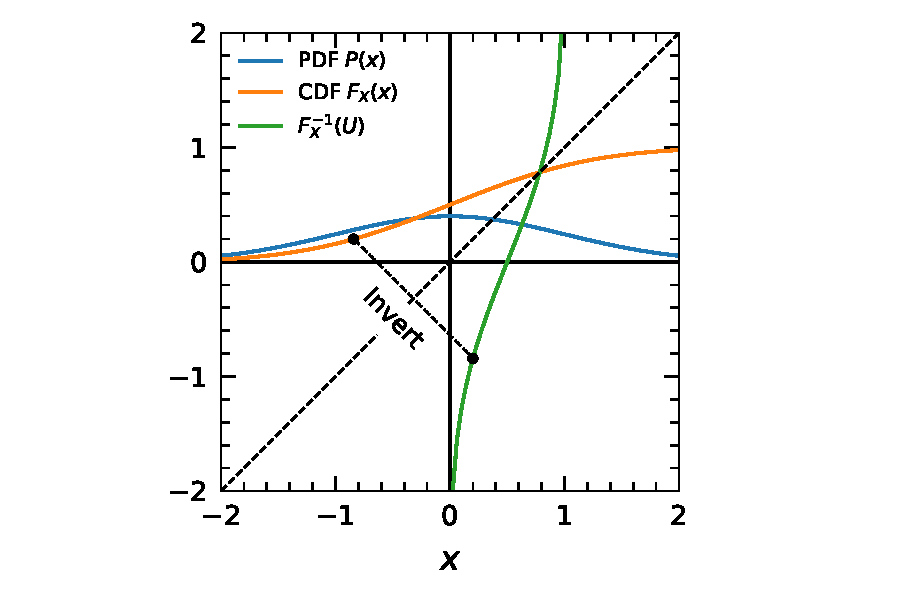
\includegraphics[width=0.7\textwidth]{figures/stats/inverse_transform_sampling_normal_dist}
\caption{
Example application of the inverse sampling method to generate the normal distribution, adapted from \href{https://en.wikipedia.org/wiki/File:Inverse_transform_sampling.png}{Olivier Ricou}.
}
\label{fig:inverse_sampling_method_normal}
\end{figure}

%%%%%%%%%%%%%%%%%%%%%%%%%%%%%%%%%%%%%%%%%%%%%%%%%%%%%%%%
\subsubsection{Rejection Sampling}
\label{additional:misc:sampling_prob_dist:reject}
% https://www.youtube.com/watch?v=OXDqjdVVePY
% TODO

